\section{What do Christopher Alexander’s (building) architectural patterns and (software) design patterns have in common? Explain with a concrete example.}

Over the ages, architectural patterns have been developed to build buildings and plan cities and these patterns have stood the test of time.
Nowadays, cities are composed of  blocks, buildings, doors, windows, roof-tops, traffic lights, stores, and people. And we walk through the city, everything : city blocks, traffic lights, doors, etc, works the way we expect. In essence, we’ve developed a pattern language which makes building new cities and towns a (mostly) trivial process. 

In software development, we can make the parallel with architectural and design patterns. Thanks to the design patterns, when someone looks at a software organization, he can feel as comfortable and familiar as he would walking on city block.

\section{Give a definition of the notion of design pattern.}

\textbf{Definition from the course}
A design pattern describes in a reusable the best practice solution to a recurring design problem. It provides a better structure and a design improved confidence. It improves also key software quality factors such as maintainability, reusability, extensibility... It promotes the reuse of components at analysis, architecture and design level. Finally, it codifies "good" analysis and designs that disseminate know-how, help novice and encourage abstraction.

\textbf{Definition from Gang of Four} \\
Design patterns are descriptions of communicating objects and classes that are customized to solve a general design problem in a particular context

\section{What are design patterns good for and why?
Why cannot you say “I have invented a design pattern”?}

Patterns provide guidance in the analysis and in the design process. Patterns reuse proven solutions from prior experiences. Patterns improve the software quality. Patterns allow a better structure and the design is improved. So the software is more maintainable, reusable, extensible... Patterns encourage also to use abstraction.

The design patterns are discovered, not invented. It takes time to emerge, to try and to improve a design pattern. We need a lot of experience to discover a pattern. And finally patterns are based on practical solutions from existing applications.


\section{Explain the different parts of which a design pattern description typically exists.
(Catchy name, Classification, Intent, Also known as, Motivation, Applicability, Structure,
Participants, Collaboration, Consequences, Implementation, Sample Code, Known
Uses, Related Patterns)}

(cf. 06-Software-Patterns, slide 56)


\begin{description}
\item[Catchy Name]

	a descriptive and unique name to help identify and refer to the pattern.

\item[Classification]

	Creational, Structural, or Behavioural (+ Class or Object).

\item[Intent]

	a description of the goal behind the pattern and the reasons for using it.

\item[Also known as]

	other names for the pattern.

\item[Motivation]

	a scenario consisting of a problem and a context in which this pattern can be used.

\item[Applicability]

	situations in which this pattern is usable; the context for the pattern.

\item[Structure]

	graphical representation of the pattern. Class diagrams and interaction diagrams can be used for this purpose.

\item[Participants]

	list of classes and objects used in the pattern and their roles in the design.

\item[Collaboration]

	how classes and objects used in the pattern interact with each other.

\item[Consequences]

	results, side effects, and trade offs caused by using the pattern.

\item[Implementation]

	implementation of the pattern; the solution part of the pattern.

\item[Sample Code]

	illustration of how the pattern can be used in a programming language.

\item[Known Uses]

	examples of real usages of the pattern.

\item[Related Patterns]

	other patterns that have some relationship with the pattern; discussion of the differences between the pattern and similar patterns.
\end{description}


\section{Explain and illustrate the Abstract Factory design pattern in detail.
Clearly mention its problem, solution, participants, structure and applicability.}

(cf. 06-Software-Patterns, slides 32-39)\\


\subsection{Problem}

We have entangled hierarchies. In other words, behaviour and visualisation of UI objects are combined in the same inheritance structure.

\begin{center}
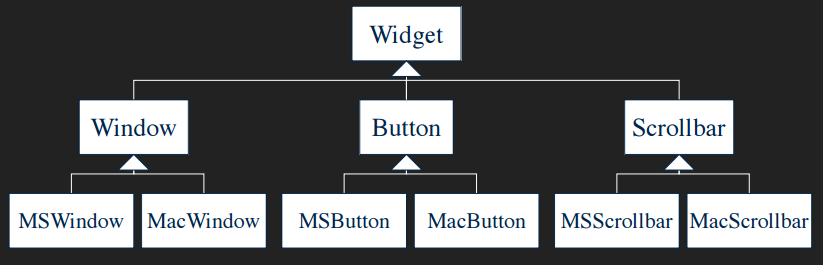
\includegraphics[width=1.0\textwidth]{06-33.png}
\end{center}



\subsection{Solution}

Separate behaviour of UI objects from their visualisation.

\begin{center}
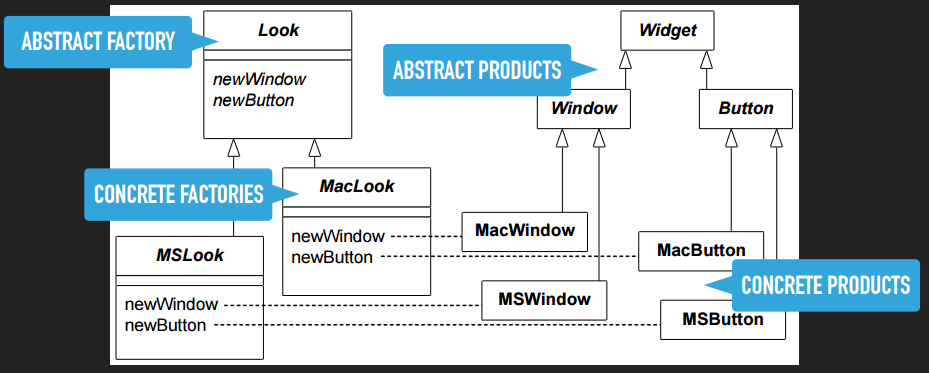
\includegraphics[width=1.0\textwidth]{06-36.png}
\end{center}



\subsection{Participants}

\begin{description}
\item[AbstractFactory]
	
	declares an interface for operations that create abstract product objects.

\item[ConcreteFactory]

	implements the operations to create concrete product objects.

\item[AbstractProduct]

	defines a product object to be create by the corresponding concrete factory.

\item[ConcreteProduct]

	defines a product object that implements the AbstractProduct interface.

\item[Client]
	
	uses only interfaces declared by AbstractFactory and AbstractProduct classes.
\end{description}



\subsection{Structure}

\begin{center}
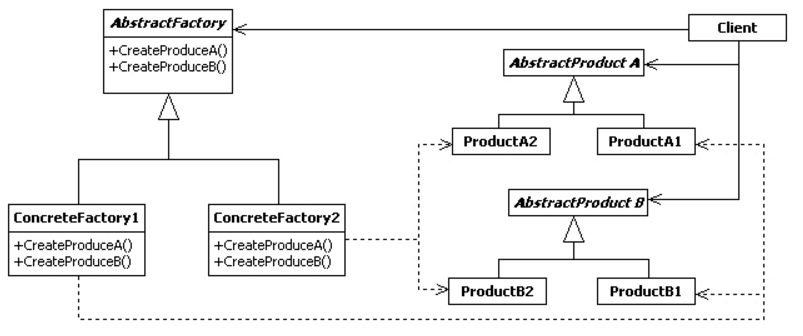
\includegraphics[width=1.0\textwidth]{06-38.png}
\end{center}

Normally a single instance of ConcreteFactory is created at run-time.



\subsection{Applicability}

This solution can be applied in general when

\begin{itemize}
\item a system should be independent of how its products are created, composed, and represented
\item a system should be configured with families of products
\item you want to provide a class library of products, and you want to reveal their interfaces, not their implementations
\item a family of related product objects is designed to be used together, and you need to enforce this constraint
\end{itemize}

\section{Explain the Factory Method design pattern in detail.
Clearly mention its Intent, Motivation, Applicability, Participants, Collaboration,
Consequences and Implementation.}

(cf. 06-Software-Patterns, slides 62-73)

\begin{description}
\item[Classification:] Object Creational.

\item[Intent:] Define an interface for creating an object, but let subclasses decide which class to instantiate. Factory Method lets a class defer instantiation to subclasses.

\item[Motivation:] Consider an application framework for creating desktop applications.
\begin{itemize}
\item Such applications work with documents.
\item The framework contains basic operations for opening, closing and saving documents.
\item Specific applications (e.g., subclasses of Application) can create their own kinds of documents (subclasses of Document)
\item For example, a DrawingApplication creates DrawingDocuments.
\item To create application-specific documents, the abstract Application class needs to delegate to its subclasses.
\end{itemize}
\end{description}

\begin{center}
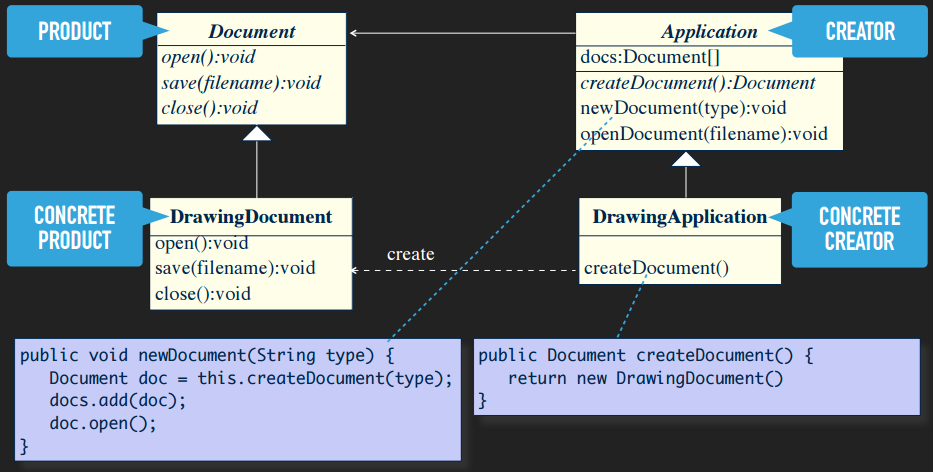
\includegraphics[width=1.0\textwidth]{06-67.png}
\end{center}


\subsection{Applicability}

Use the Factory Method design pattern when:


\begin{itemize}
\item A class can't anticipate the class of objects it must create.
\item A class wants its subclasses to specify the obvjects it creates.
\item Classes delegate responsibility to one of several helper subclasses, and you want to localise the knowledge of which helper classes to use.
\end{itemize}

\subsection{Participants}

\begin{description}
\item[Product]
	
	defines the interface of objects the factory method creates.

\item[ConcreteProduct]

	implements the Product interface.

\item[Creator]
	
	declares the abstract factory method (createDocument), and may call the factory method to create a Product object.

\item[ConcreteCreator]
	
	overrides factory method with a concrete one to return a ConcreteProduct instance.
\end{description}

\subsection{Collaborations}

Creator relies on its ConcreteCreator subclasses to specify the concrete factory method, so that it returns an instance of the appropriate ConcreteProduct.


\subsection{Consequences}

It is more reusable than creating objects directly, and it connects parallel class hierarchies.

\begin{center}
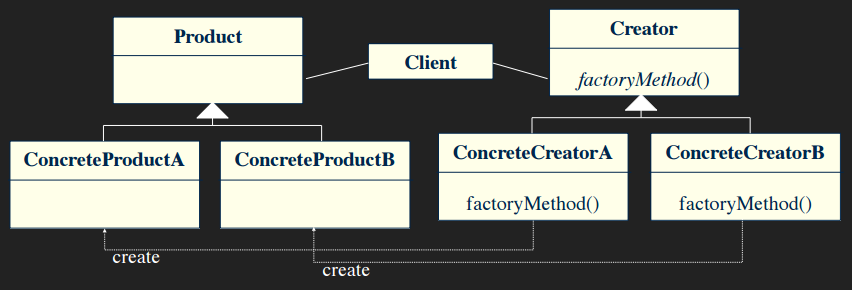
\includegraphics[width=1.0\textwidth]{06-71.png}
\end{center}

\subsection{Implementation}

\begin{description}
\item[Variation 1]

	Some factory methods can provide a default. In that case, the factory method is not abstract

\item[Variation 2]
	
	Factory method can be parametrised to return multiple kinds of products, e.g. pass an extra parameter to createDocument to specify the kind of Document to create.
\end{description}


\section{Same question as previous one but for one of the following design patterns:
Strategy and Decorator}

Strategy: (cf. 06-Software-Patterns, slides 74-84)
\\
Decorator: (cf. 06-Software-Patterns, slides 85-95)

\subsection{Strategy}

\vspace{12pt}\textbf{Classification:}\\
Object Behavioural.

\vspace{12pt}\textbf{Intent:}\\
Define a family of algorithms, encapsulate each one, and make them interchangeable. Strategy lets the algorithm vary independently from clients that use it.

\vspace{12pt}\textbf{Motivation:}\\
Different sorting algorithms, String search in a text processor, etc.

There are common situations when classes differ only in their behaviour. For such cases, it is a good idea to isolate the algorithms in separate classes in order to have the ability to select different algorithms at runtime.


\vspace{12pt}\textbf{Applicability:}\\

Use the Strategy design pattern when:


\begin{itemize}
\item Many related classes that differ only in their behaviour.
\item You need different variants of an algorithm.
\item An algorithm uses data that clients should not know about.
\item A class defines many behaviours.
\end{itemize}

\vspace{12pt}\textbf{Participants:}\\


\begin{description}
\item[Strategy]

	declares an interface common to all supported algorithms. Context uses this interface to call the algorithm defined by a ConcreteStrategy.

\item[ConcreteStrategy]

	implements the algorithm using the Strategy interface.

\item[Context]

	is configured with a ConcreteStrategy object, maintains a reference to a Strategy object, and may define an interface that lets Strategy access its data.

\end{description}

\begin{center}
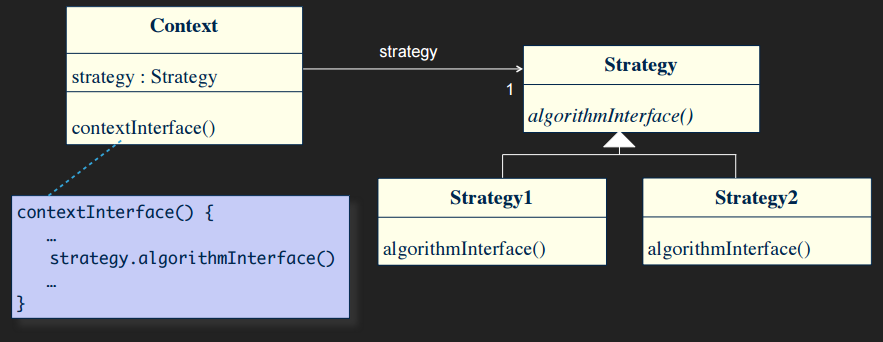
\includegraphics[width=1.0\textwidth]{06-81.png}
\end{center}

\vspace{12pt}\textbf{Collaborations:}\\

Strategy and Context interact to implement the chosen algorithm.

\begin{itemize}
\item Context may pass all data required by the algorithm to the strategy when the algorithm is called.
\item Context can pass itself as an argument to Strategy operations.
\end{itemize}

A Context forwards requests from its clients to its strategy. Clients usually create and pass a ConcreteStrategy object to the Context. From then, they interact with the Context exclusively.

\vspace{12pt}\textbf{Consequences:}\\

\begin{itemize}
\item Families of related algorithms.
\item An alternative to subclassing.
\item Strategies eliminate conditionals.
\item Provide a choice of implementation, which allow for different implementations of same behaviour.
\item Overhead involved from communication between Context and Strategy, and increased number of objects.
\end{itemize}

\vspace{12pt}\textbf{Implementation:}\\

The Strategy interface must provide enough information to ConcreteStrategy.

Default behaviour can be incorporated in the Context object. If no strategy object is present, this default behaviour can be used.

\subsection{Decorator}

\vspace{12pt}\textbf{Classification:}\\

Object Structural.



\vspace{12pt}\textbf{Intent:}\\

Attach additional responsibilities to an object dynamically. Decorators provide a dynamic alternative for subclassing.



\vspace{12pt}\textbf{Motivation:}\\

Adding borders/scrollbars/... to a visual component.

When traditional solutions are impractical for:


\begin{itemize}
\item When I want to apply different decorations to a same component.
\item When I want to apply a same decoration to a different components.
\end{itemize}



\vspace{12pt}\textbf{Applicability:}\\

Use the Decorator design pattern:


\begin{itemize}
\item To add responsibilities to individual objects dynamically and transparently without affecting other objects.
\item For responsibilities that can be withdrawn.
\item When extending by subclassing is impractical.
\end{itemize}




\vspace{12pt}\textbf{Participants:}\\

\begin{description}
\item[Component]

	defines the interface for objects that can have responsibilities added to them dynamically.

\item[ConcreteComponent]

	defines an object to which we want to attach additional responsibilities.

\item[Decorator]

	maintains a reference to a Component object and defines an interface that conforms to the Components interface.

\item[ConcreteDecorator]

	adds responsibilities to the component.
\end{description}

\begin{center}
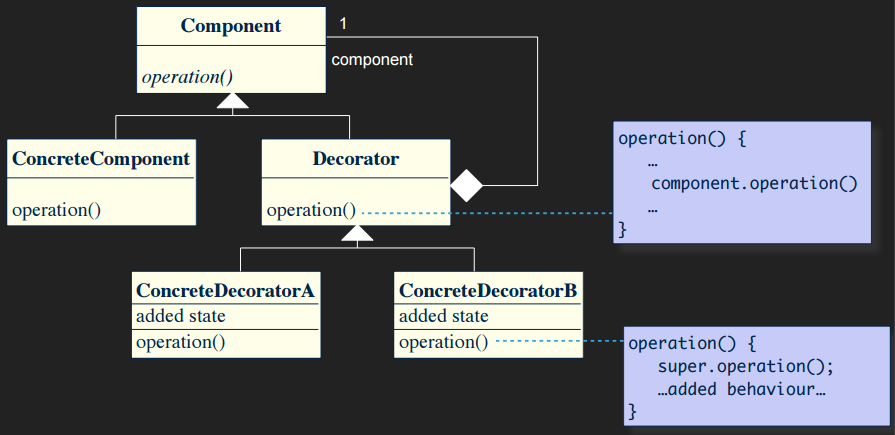
\includegraphics[width=1.0\textwidth]{06-92.png}
\end{center}


\vspace{12pt}\textbf{Collaborations:}\\

Decorator forwards requests to the Component object. It may optionally perform additional behaviour before and after forwarding the request.




\vspace{12pt}\textbf{Consequences:}\\


\begin{itemize}
\item More flexible than static inheritance, as it is possible to dynamically add or withdraw responsibilities.
\item Avoids classes with a lot of features.
\item Lots of little objects.
\end{itemize}



\vspace{12pt}\textbf{Implementation:}\\

Object identity can be a problem, as a decorated component is not identical to the object itself.


\section{What is an antipattern? How does it compare to a design pattern? What purpose does it
serve?}

(cf. 06-Software-Patterns, slides 97-98)\\

Design patterns identify \textbf{good working practices}.

Anti patterns identify \textbf{common mistakes} and how these mistakes can be overcome in refactored solutions.

An AntiPattern is \textit{"a commonly used solution to a problem that generates decidedly negative consequences"}.

An AntiPattern is a special (negative) design pattern which features an extra refactored solution to the problem.


\section{What is an antipattern? Explain at least 4 of the 7 deadly sins related to antipatterns.}

(cf. 06-Software-Patterns, slides 100-101)\\

\begin{description}
\item[Haste:]

	Hasty decisions lead to compromises in software quality. Especially testing is a victim.

	\textit{"Just clean up the code, we ship tomorrow..."}
    
\item[Apathy:]

	Not caring about solving known problems.

	\textit{"Reuse? Who's ever gonna reuse this crappy code?"}

\item[Narrow-mindedness:]

	Refusal to practice solutions that are widely known to be effective.

	\textit{"I don't need to know, and... I don't care to know"}

\item[Sloth (lazyness):]

	Making poor decisions based upon easy answers (lazy developers).

\item[Avarice (greed):]

	The modeling of excessive details, resulting in overcomplexity due to insufficient abstract.

	\textit{"I'm impressed! The most complex model ever done!"}

\item[Ignorance:]

	Failing to seek understanding.

	\textit{"100 pages... let's find a one page summary on the net"}

\item[Pride:]
	
	Reinventing designs instead of reusing them.
\end{description}

\section{Explain The Blob antipattern.}

(cf. 06-Software-Patterns, slides 103-106)\\

\begin{description}
\item[Category:]
	
	Software Development.

\item[Also Known As:]

	The God Class.

\item[Scale:]

	Application.

\item[Refactored Solution Name:]

	Refactoring of Responsibilities.

\item[Root Causes:]

	Sloth, Haste.
\end{description}



\subsection{General Form}

\begin{itemize}
\item Designs where one class monopolises the processing, and other classes primarily encapsulate data.
\item The key problem is that the majority of responsibilities is allocated to a single class.
\item In general, it is a kind of procedural design which conflicts with Object-Oriented paradigm.
\end{itemize}



\subsection{Refactored Solution}

\begin{itemize}
\item Identify or categorise related attributes and operations.
\item Look for "natural homes" for these collections of functionality.
\item Apply OO design techniques (e.g., inheritance, ...).
\item Apply refactorings to bring code back in shape.
\end{itemize}
